\section{CADO: Computer Aided Design Optimization Tool}
CADO is the tool of choice to realize a one click CAD-to-Topology-Optimization-back-to-CAD experience. With CADO, the user only has to select the input file on which to apply the topology optimization and set the parameters which for example define the resolution or refinement level. By executing the \texttt{Run} command the tool starts the pipeline illustrated in \autoref{fig:pipeline}: 

From the given geometry (a) we start off by voxelizing (b). Next, topology optimization is applied (c) and the surface points are computed (d). After extracting the NURBS surface (e), finally, the boolean operation is executed which results in the final geometry (f). All of this is achieved without further user interaction. To get a better insight into the implementation, in the next sections we explain the different steps in more detail.
\begin{figure}[ht]
\begin{center}
		\begin{tikzpicture}[remember picture, auto,
    block/.style={
      rectangle,
      draw=blue,
      thick,
      fill=blue!20,
      text width=5em,
      align=center,
      rounded corners,
      minimum height=2em
    },
    block1/.style={
      rectangle,
      draw=blue,
      thick,
      fill=blue!20,
      text width=5em,
      align=center,
      rounded corners,
      minimum height=2em
    },
    line/.style={
      draw,thick,
      -latex',
      shorten >=2pt
    },
    cloud/.style={
      draw=red,
      thick,
      ellipse,
      fill=red!20,
      minimum height=1em
    }]
        \node [anchor=north,inner sep=0pt] [xshift=-4cm,yshift=0.7cm,inner sep=0pt](N1)
                {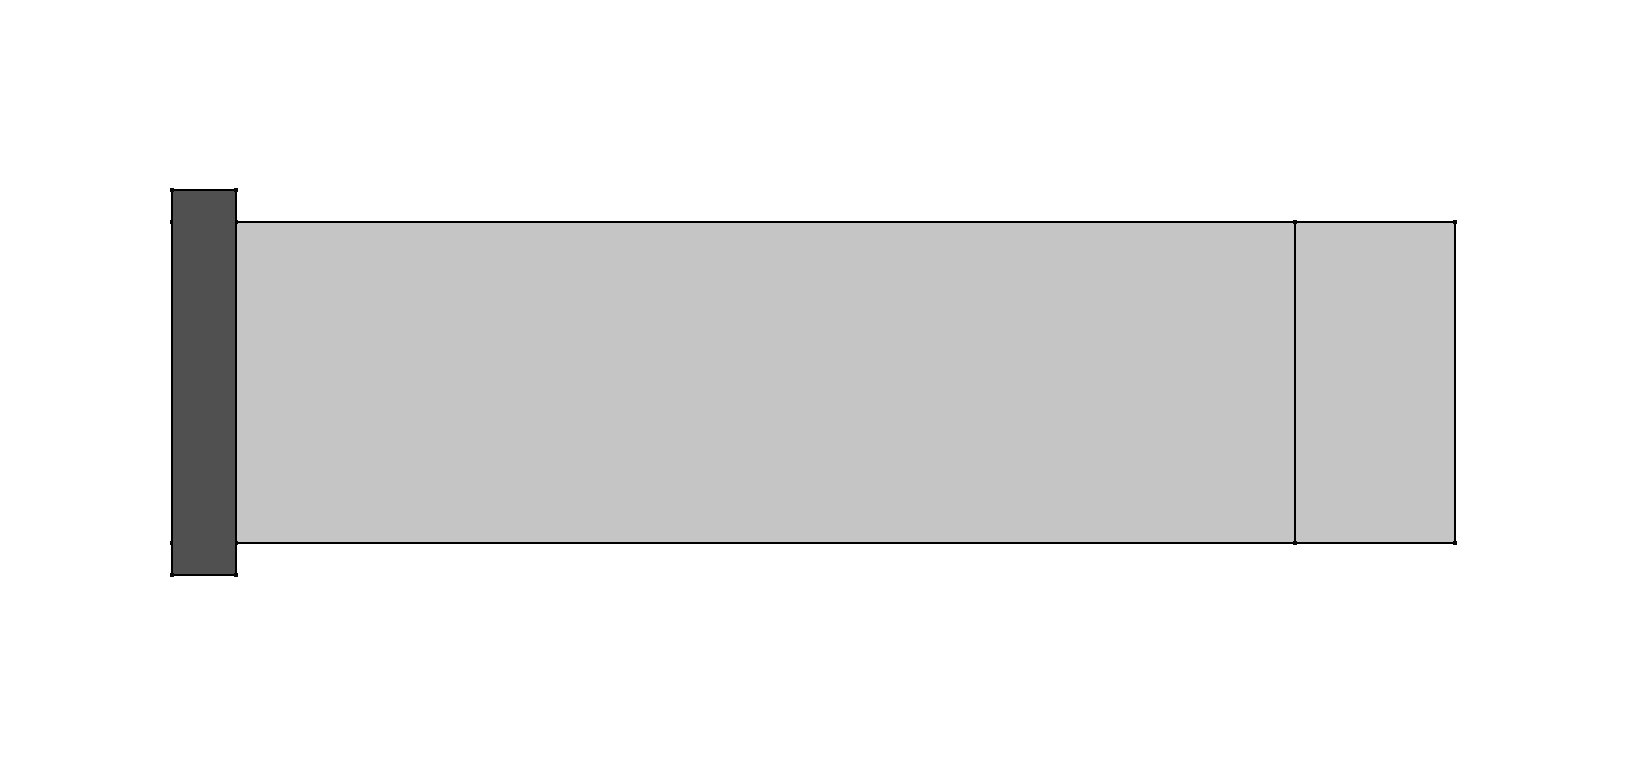
\includegraphics[scale=0.1]{Pictures/CADO_Overview/Back2CAD1.png}};
        \node [below =of N1,inner sep=0pt] [xshift=0cm,yshift=-0cm,inner sep=0pt](N5)
				{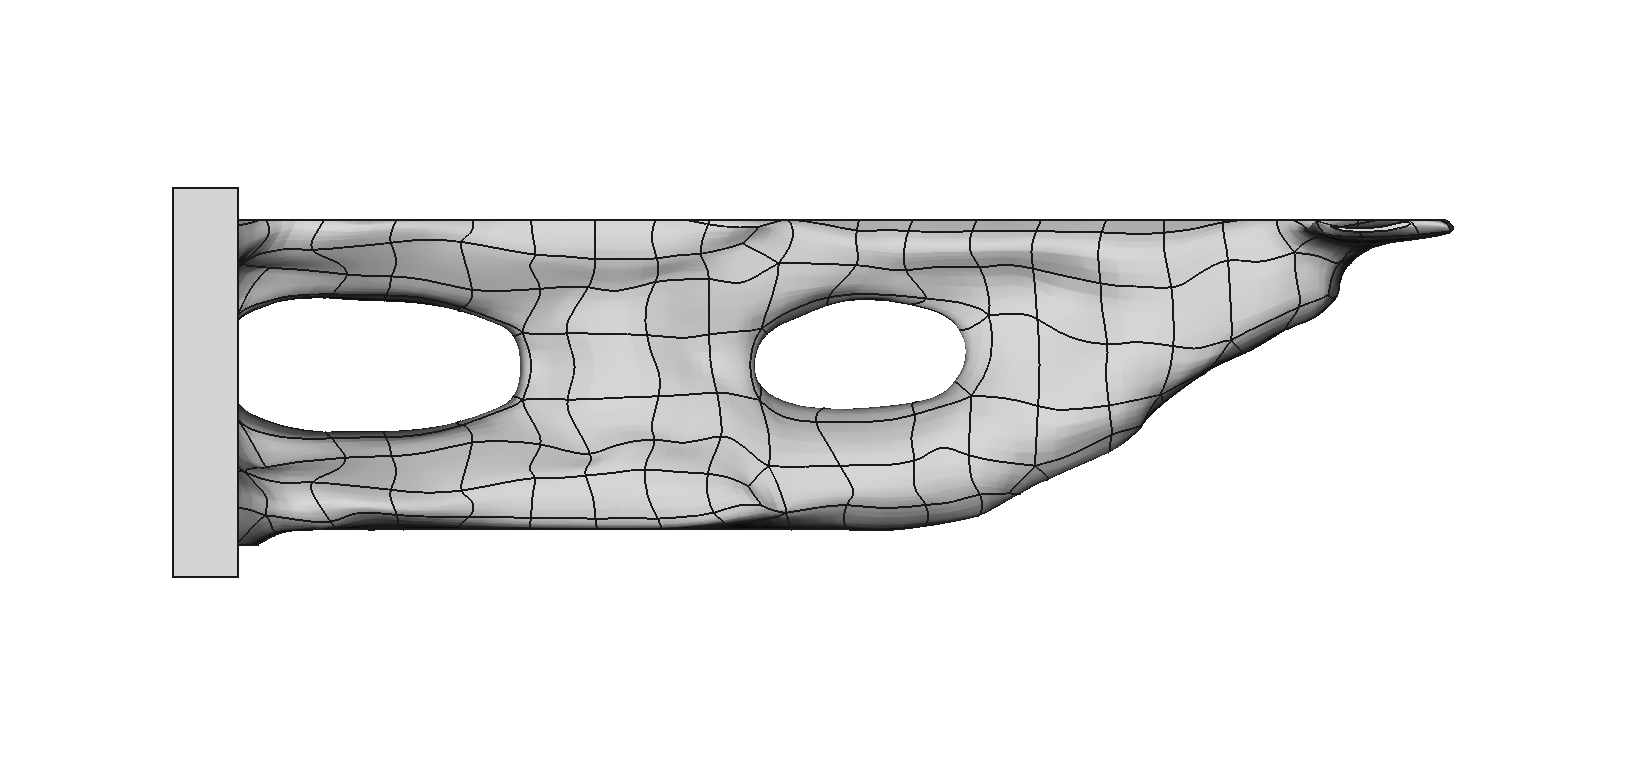
\includegraphics[scale=0.1]{Pictures/CADO_Overview/Back2CAD6.png}};
      	%\path[thick, ->,] (N5) edge [bend left] (N1); %node[yshift=-1.8cm, xshift = -0.1cm]{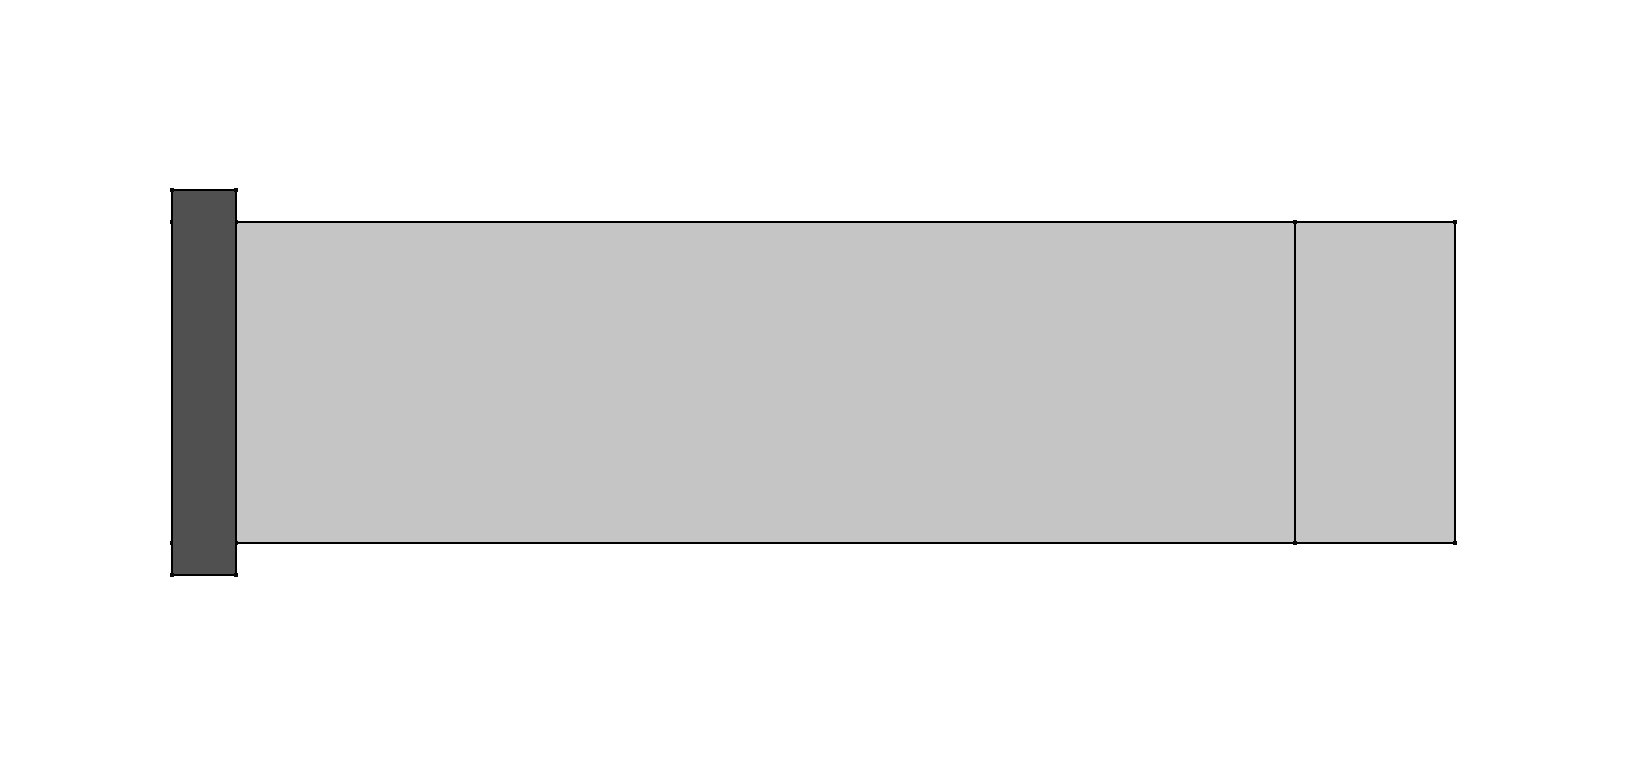
\includegraphics[scale=0.1]{Pictures/CADO_Overview/Back2CAD1.png}};
        \node [right =of N1,inner sep=0pt] [xshift=-2.5cm,yshift=3cm, inner sep=0pt](N2)             
                {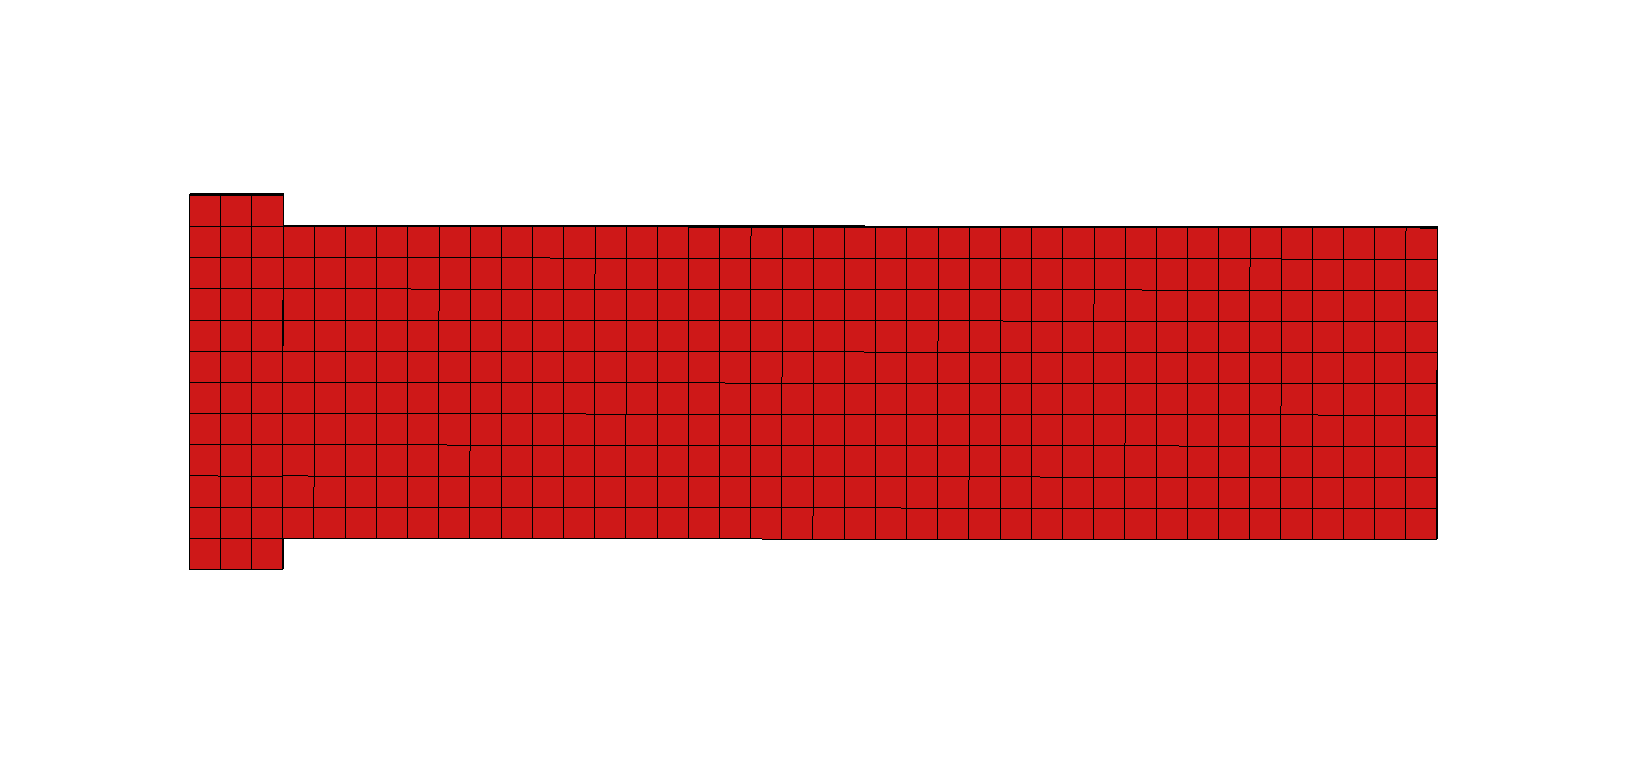
\includegraphics[scale=0.1]{Pictures/CADO_Overview/Back2CAD2.png}};
        \path[thick, ->] (N1) edge [bend left] (N2) node[yshift=0cm, xshift = -2.7cm]{(a)};
        \node [right =of N2,inner sep=0pt] [xshift=-2cm,yshift=-3cm, inner sep=0pt](N3) 
                {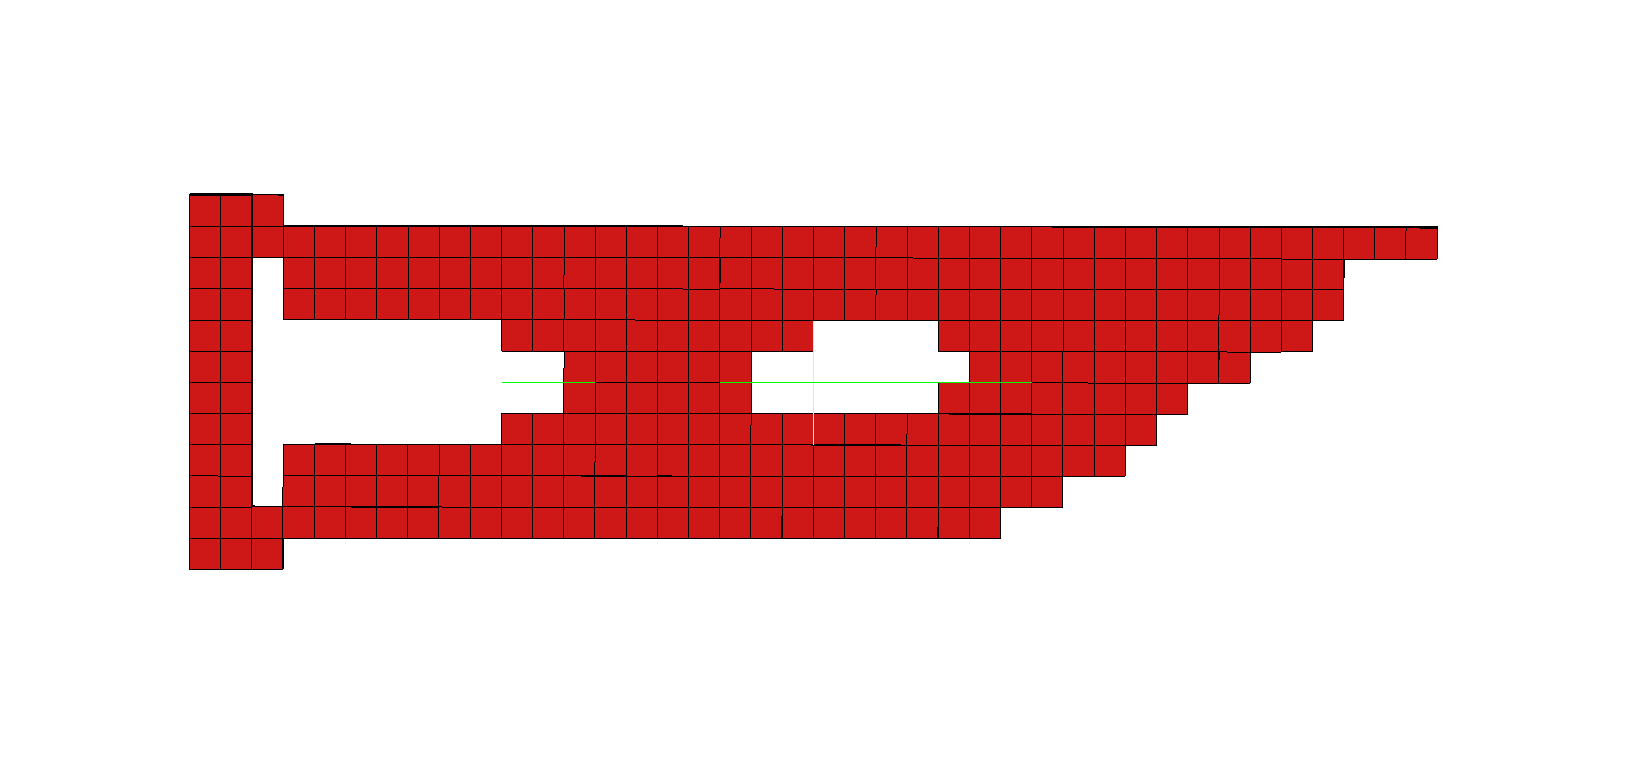
\includegraphics[scale=0.1]{Pictures/CADO_Overview/Back2CAD3.png}};
        \path[thick, ->] (N2) edge [bend left] (N3) node[yshift=1cm, xshift = 0.1cm]{(b)};
        \node [below =of N3,inner sep=0pt] [xshift=-0cm,yshift=-0cm, inner sep=0pt](N4)
                {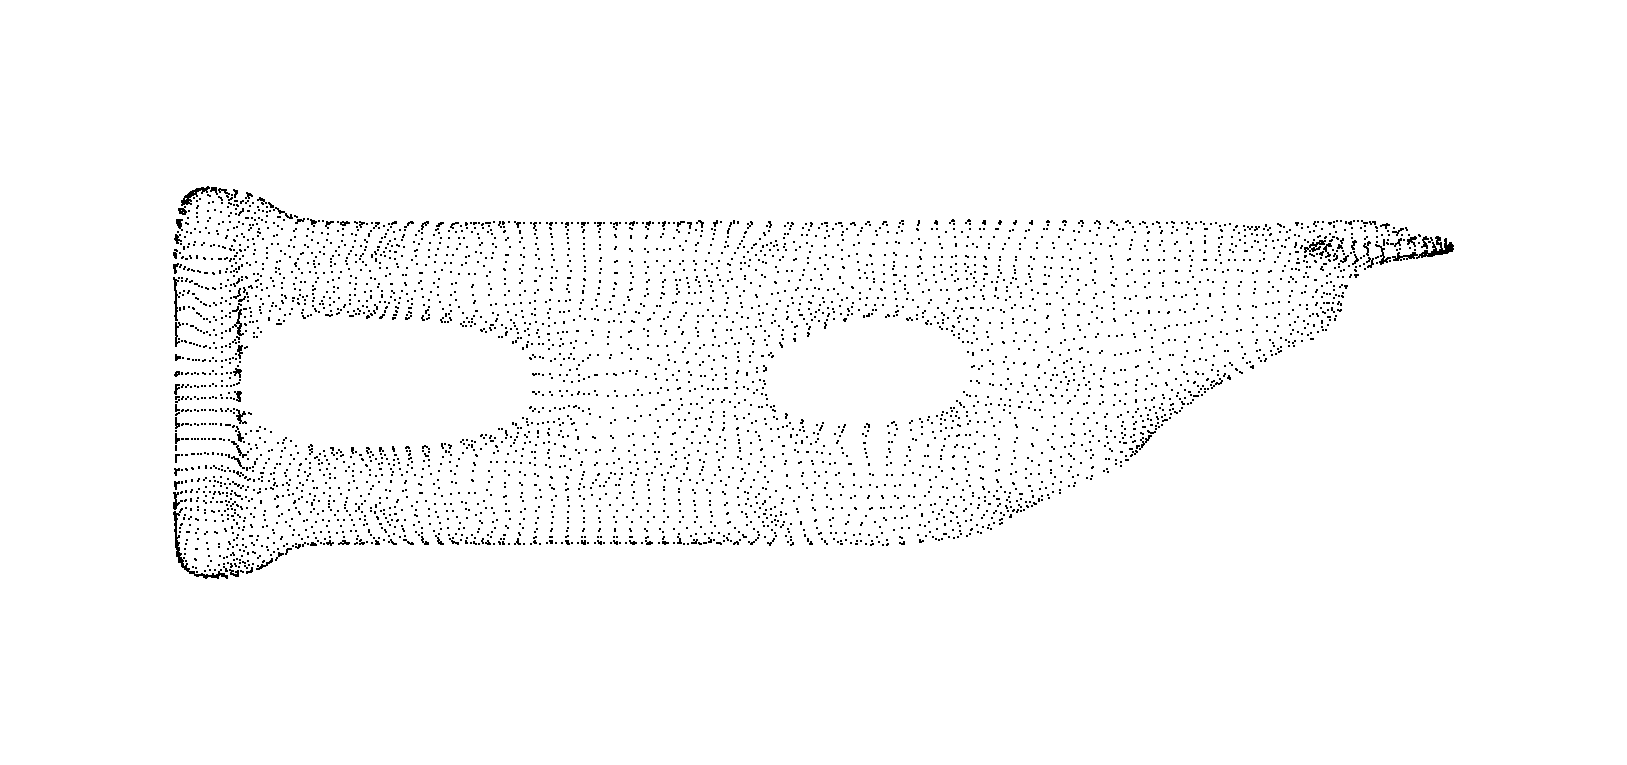
\includegraphics[scale=0.1]{Pictures/CADO_Overview/Back2CAD4.png}};
        \coordinate (N31) at (-0.7,-1);
        \coordinate (N32) at ($(N3)+(N31)$);
        \coordinate (N41) at (-0.7,1);
        \coordinate (N42) at ($(N4)+(N41)$);
        \draw[thick, ->] (N32) -- (N42) node[yshift=2.8cm, xshift = 3.4cm]{(c)};
        \node [right =of N5,inner sep=0pt] [xshift=-2.2cm,yshift=-3cm, inner sep=0pt](N6)
                {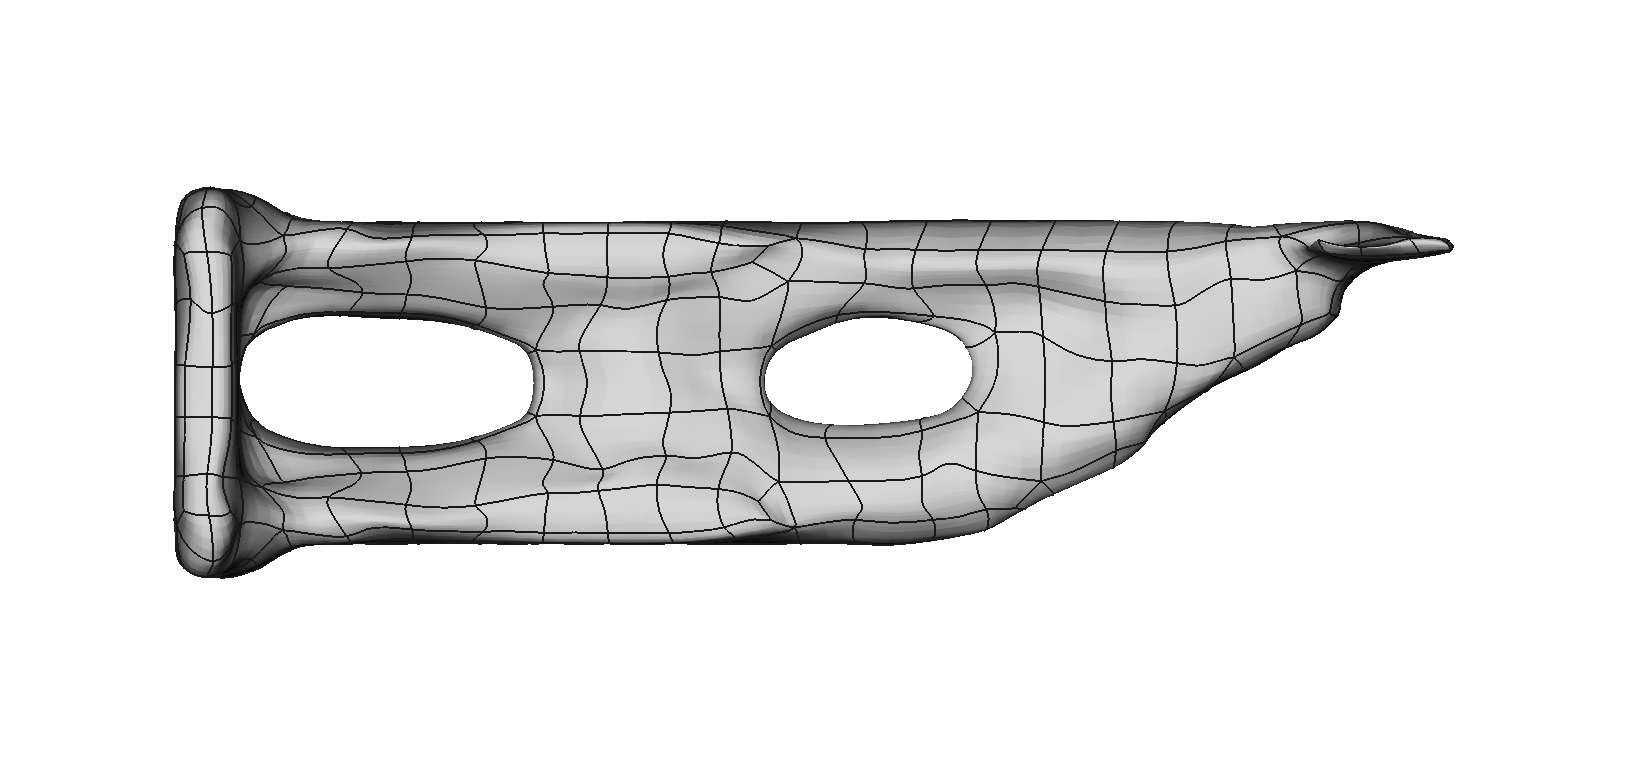
\includegraphics[scale=0.1]{Pictures/CADO_Overview/Back2CAD5.png}};
        \path[thick, ->] (N4) edge [bend left] (N6) node[yshift=0cm, xshift = 2.7cm]{(d)};
        \path[thick, ->] (N6) edge [bend left] (N5) node[yshift=-1cm, xshift = 0.1cm]{(e)} node[yshift=3cm, xshift = -7.22cm]{(f)};
        \end{tikzpicture}
        \caption{The workflow of CADO}
        \label{fig:pipeline}
	\end{center}
\end{figure}